\documentclass{article}

\usepackage[margin=1in]{geometry}
\usepackage{graphicx}

\graphicspath{ {./../figures/} }

\title{Assignment 1}
\author{Vignesh M Pai (20211132)}

\begin{document}

\maketitle

\section*{1. g)}

\begin{center}
    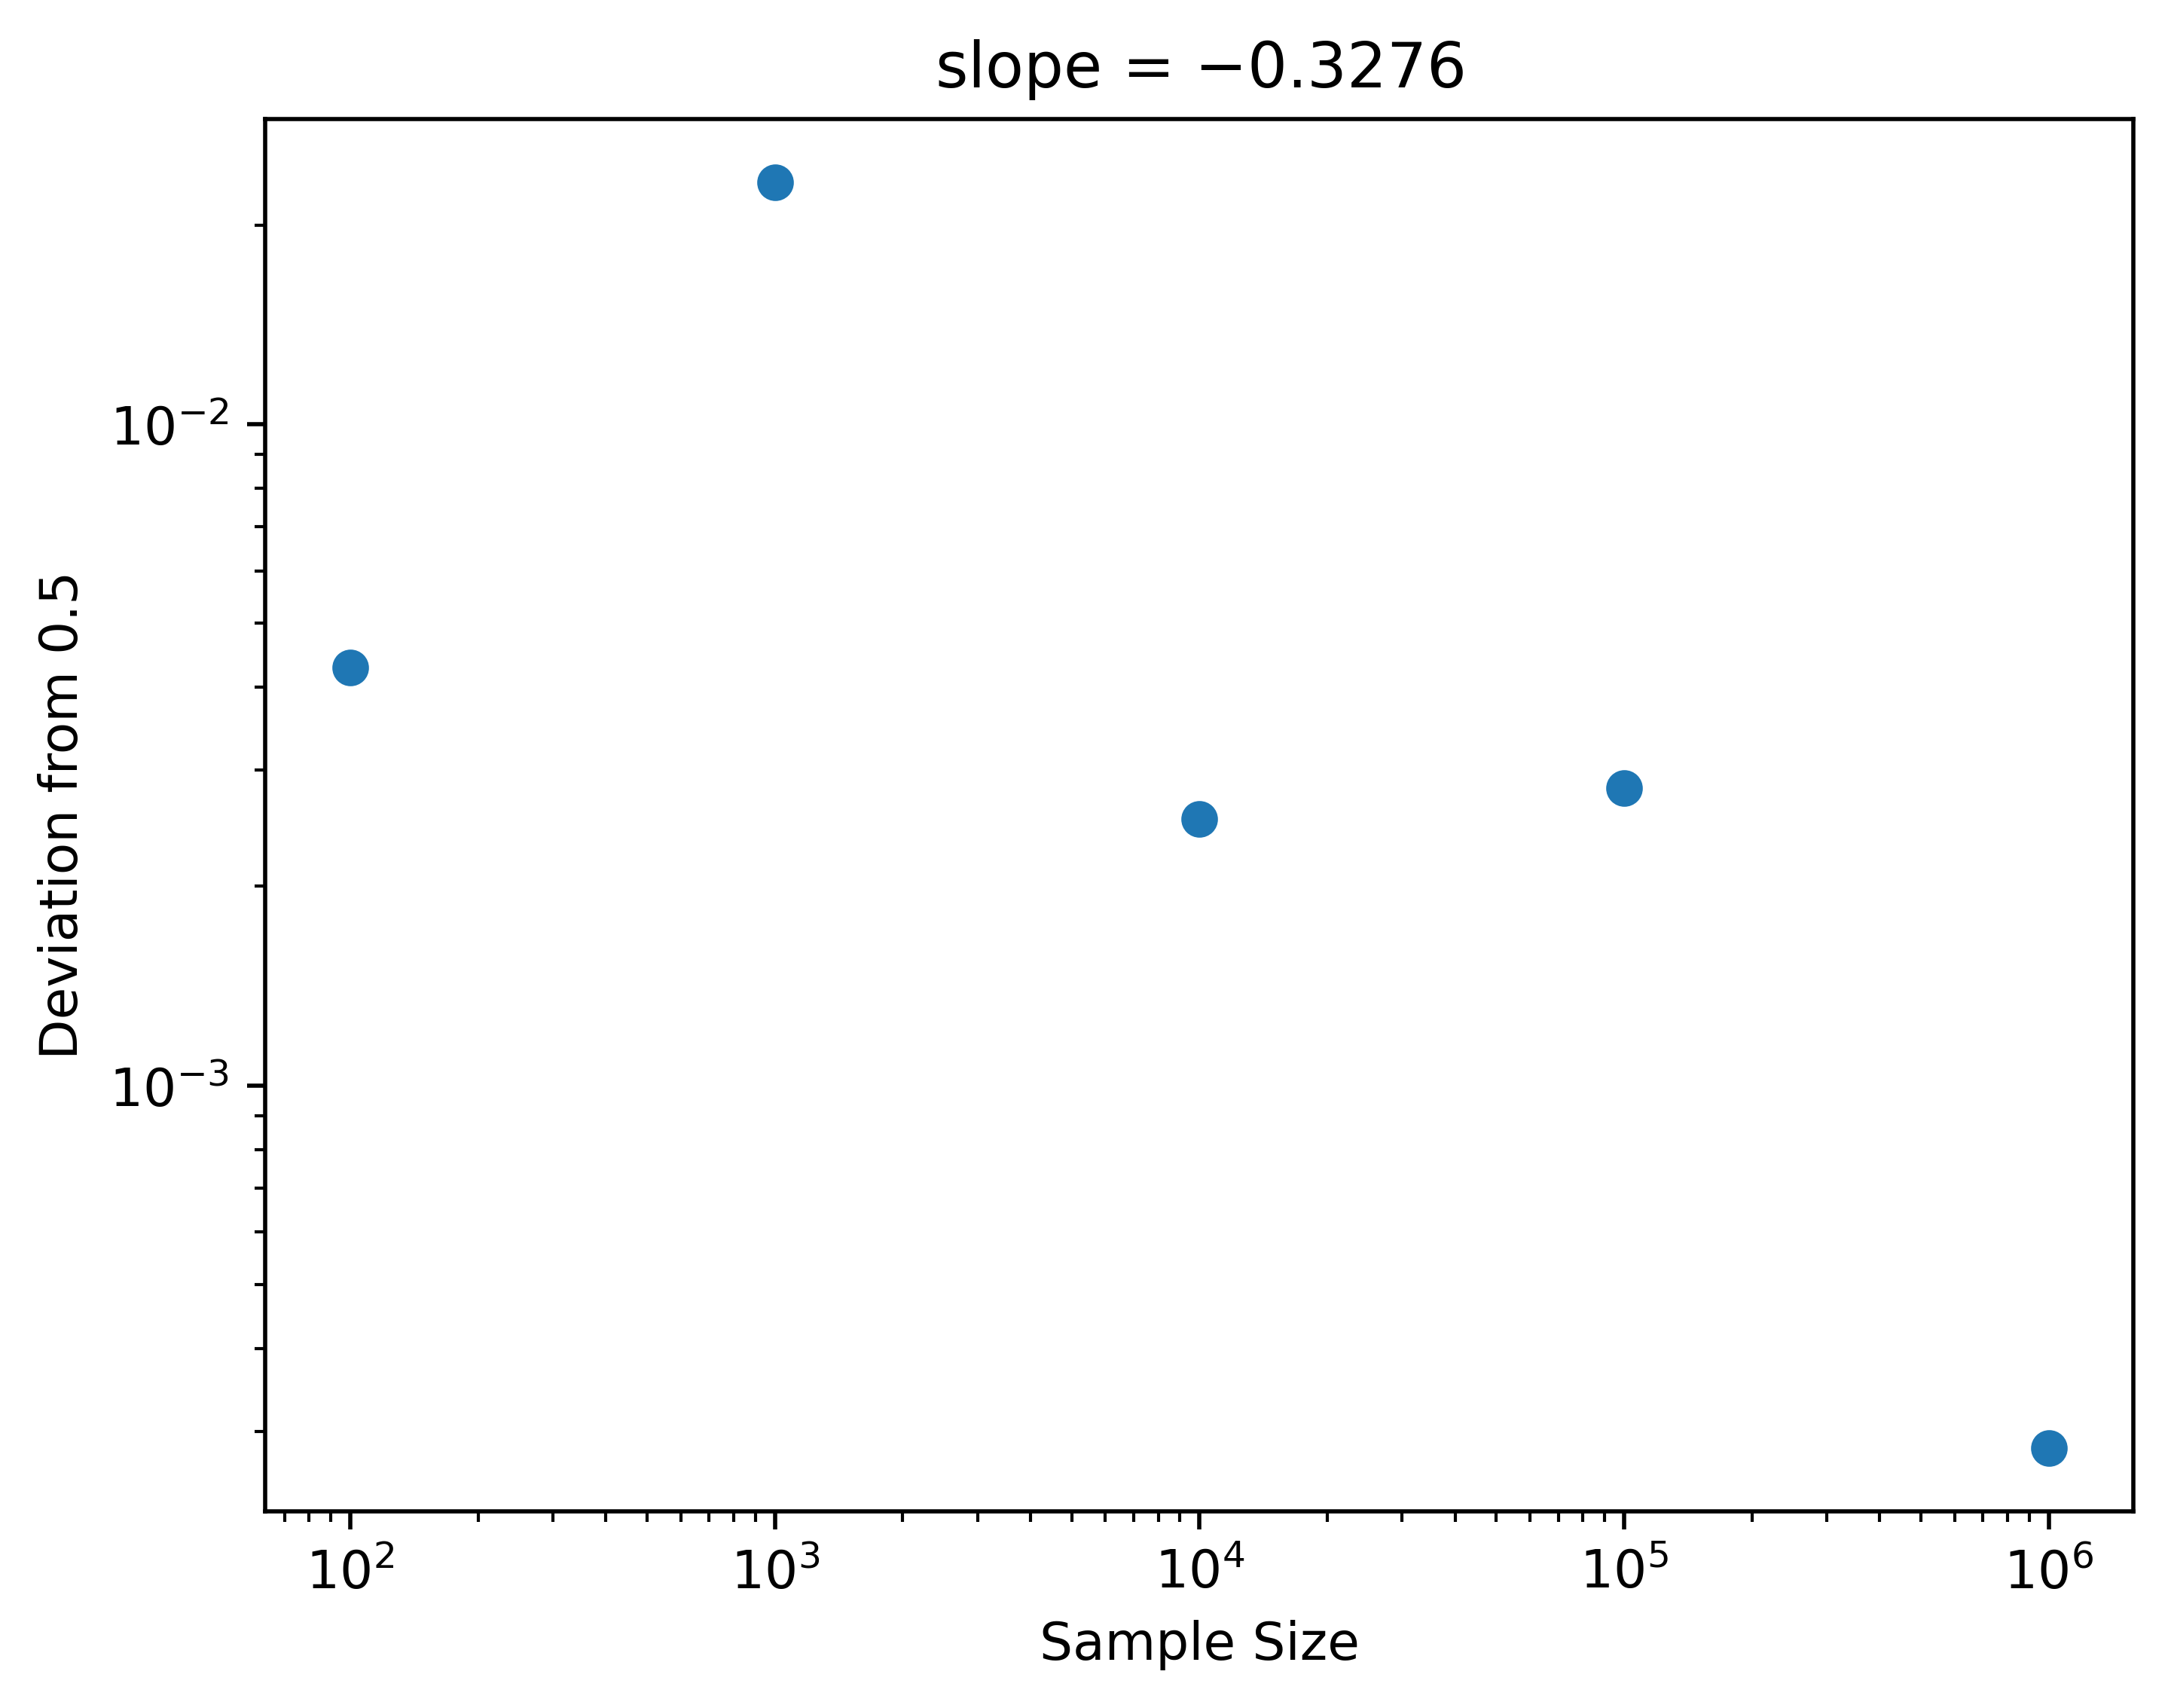
\includegraphics[scale=0.7]{1g.png}    
\end{center}

The deviation of the average from the expectation falls off as $N^{-1/2}$ where $N$ is the count.
This follows from CLT which states that the standard deviation of the sample mean falls at this same rate.

\section*{1. h)}

\begin{center}
    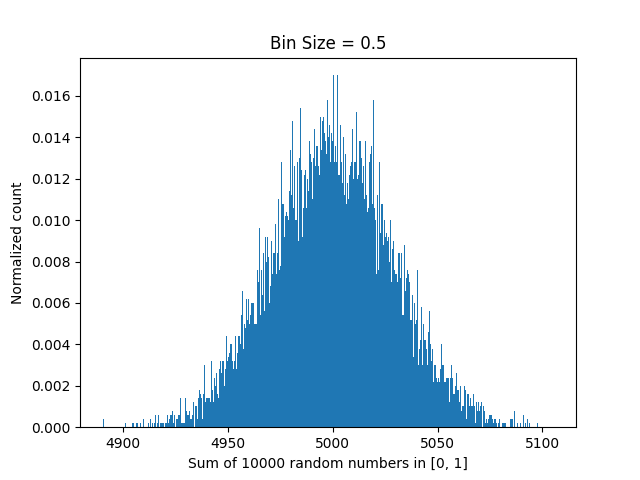
\includegraphics[scale=0.8]{1h_dx_0_5.png}

    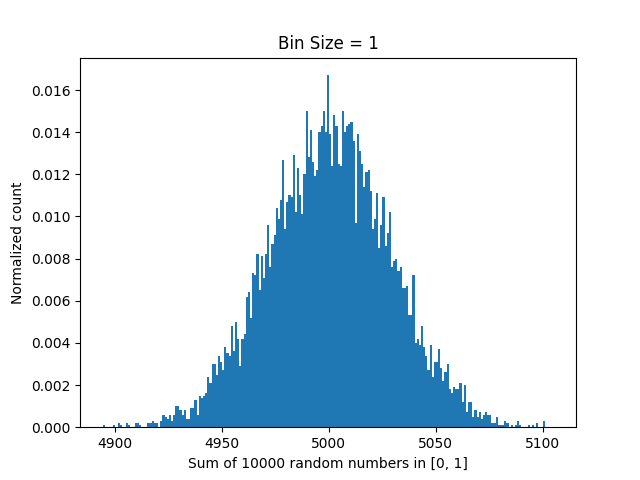
\includegraphics[scale=0.8]{1h_dx_1.png}
    
    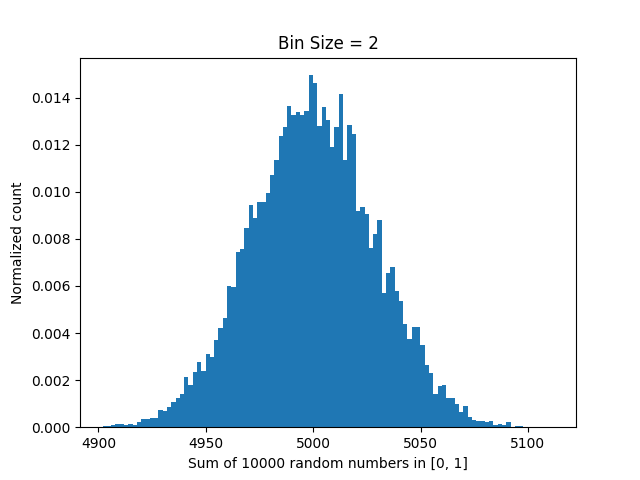
\includegraphics[scale=0.8]{1h_dx_2.png}
\end{center}

Increasing the bin size reduces the spikes in the distribution and makes it appear smoother.

\begin{center}
    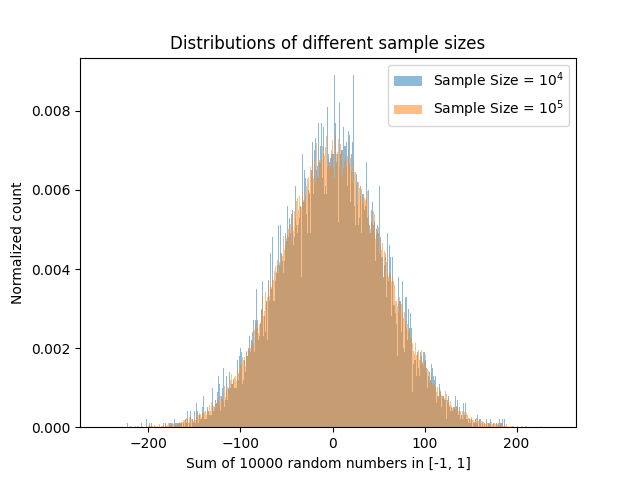
\includegraphics[scale=0.8]{1h_sample.png}        
\end{center}

The mean and standard deviations in larger samples appears to be similar, however the distribution with more samples is smoother.

\section*{1. i)}

\begin{center}
    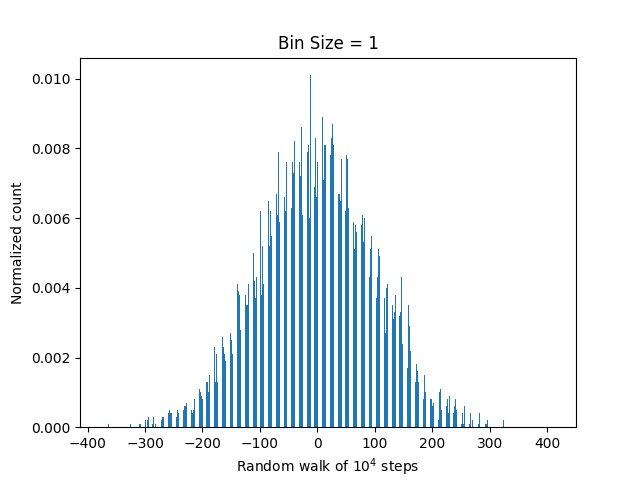
\includegraphics[scale=0.8]{1ij_dx_1.png}
\end{center}

Alternate bins in the distribution are empty, this is because we have taken an even number of steps, thus the endpoint must be even.
Hence, bins such as $[1, 2)$ will be empty. To make up for these bins, bins such as $[0, 1)$ will have twice the count estimated by CLT.

\section*{1. j)}

\begin{center}
    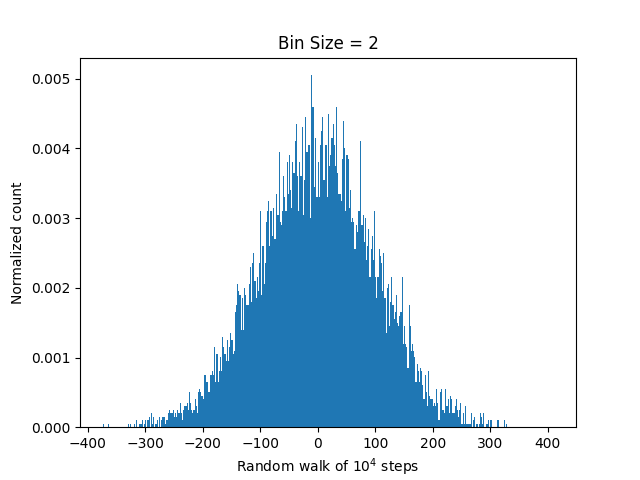
\includegraphics[scale=0.8]{1ij_dx_2.png}

    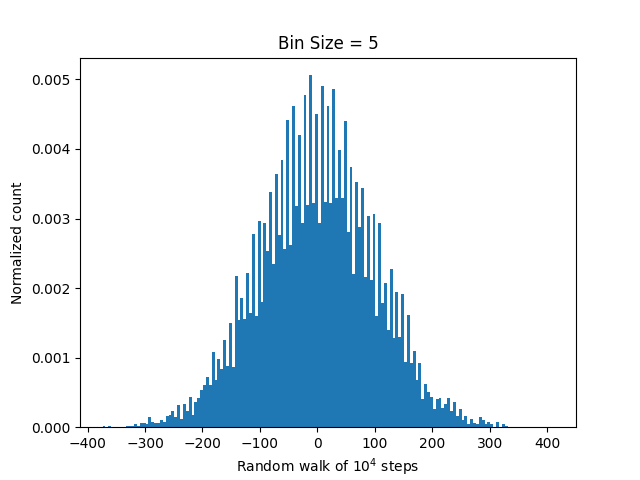
\includegraphics[scale=0.8]{1ij_dx_5.png}

    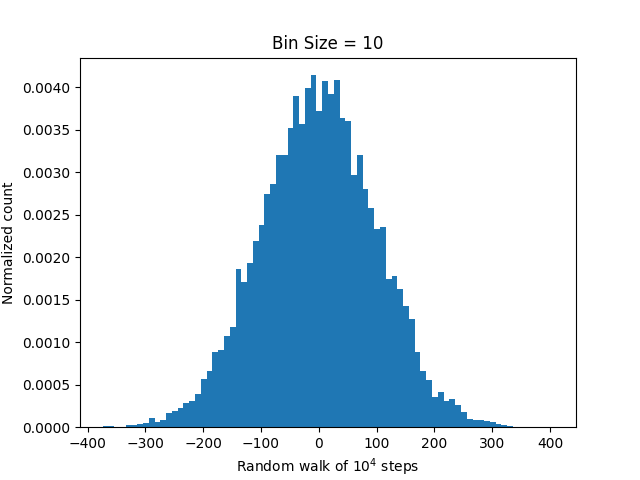
\includegraphics[scale=0.8]{1ij_dx_10.png}
\end{center}

These larger bin size distribution do not have the properties of bin size $1$.

\begin{center}
    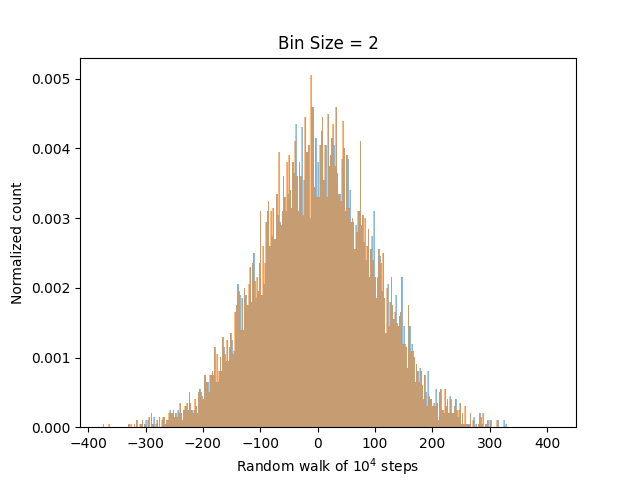
\includegraphics[scale=0.8]{1ij_shifted.png}
\end{center}

Shifting the bins shifts the histogram.

\section*{1. k)}

\begin{center}
    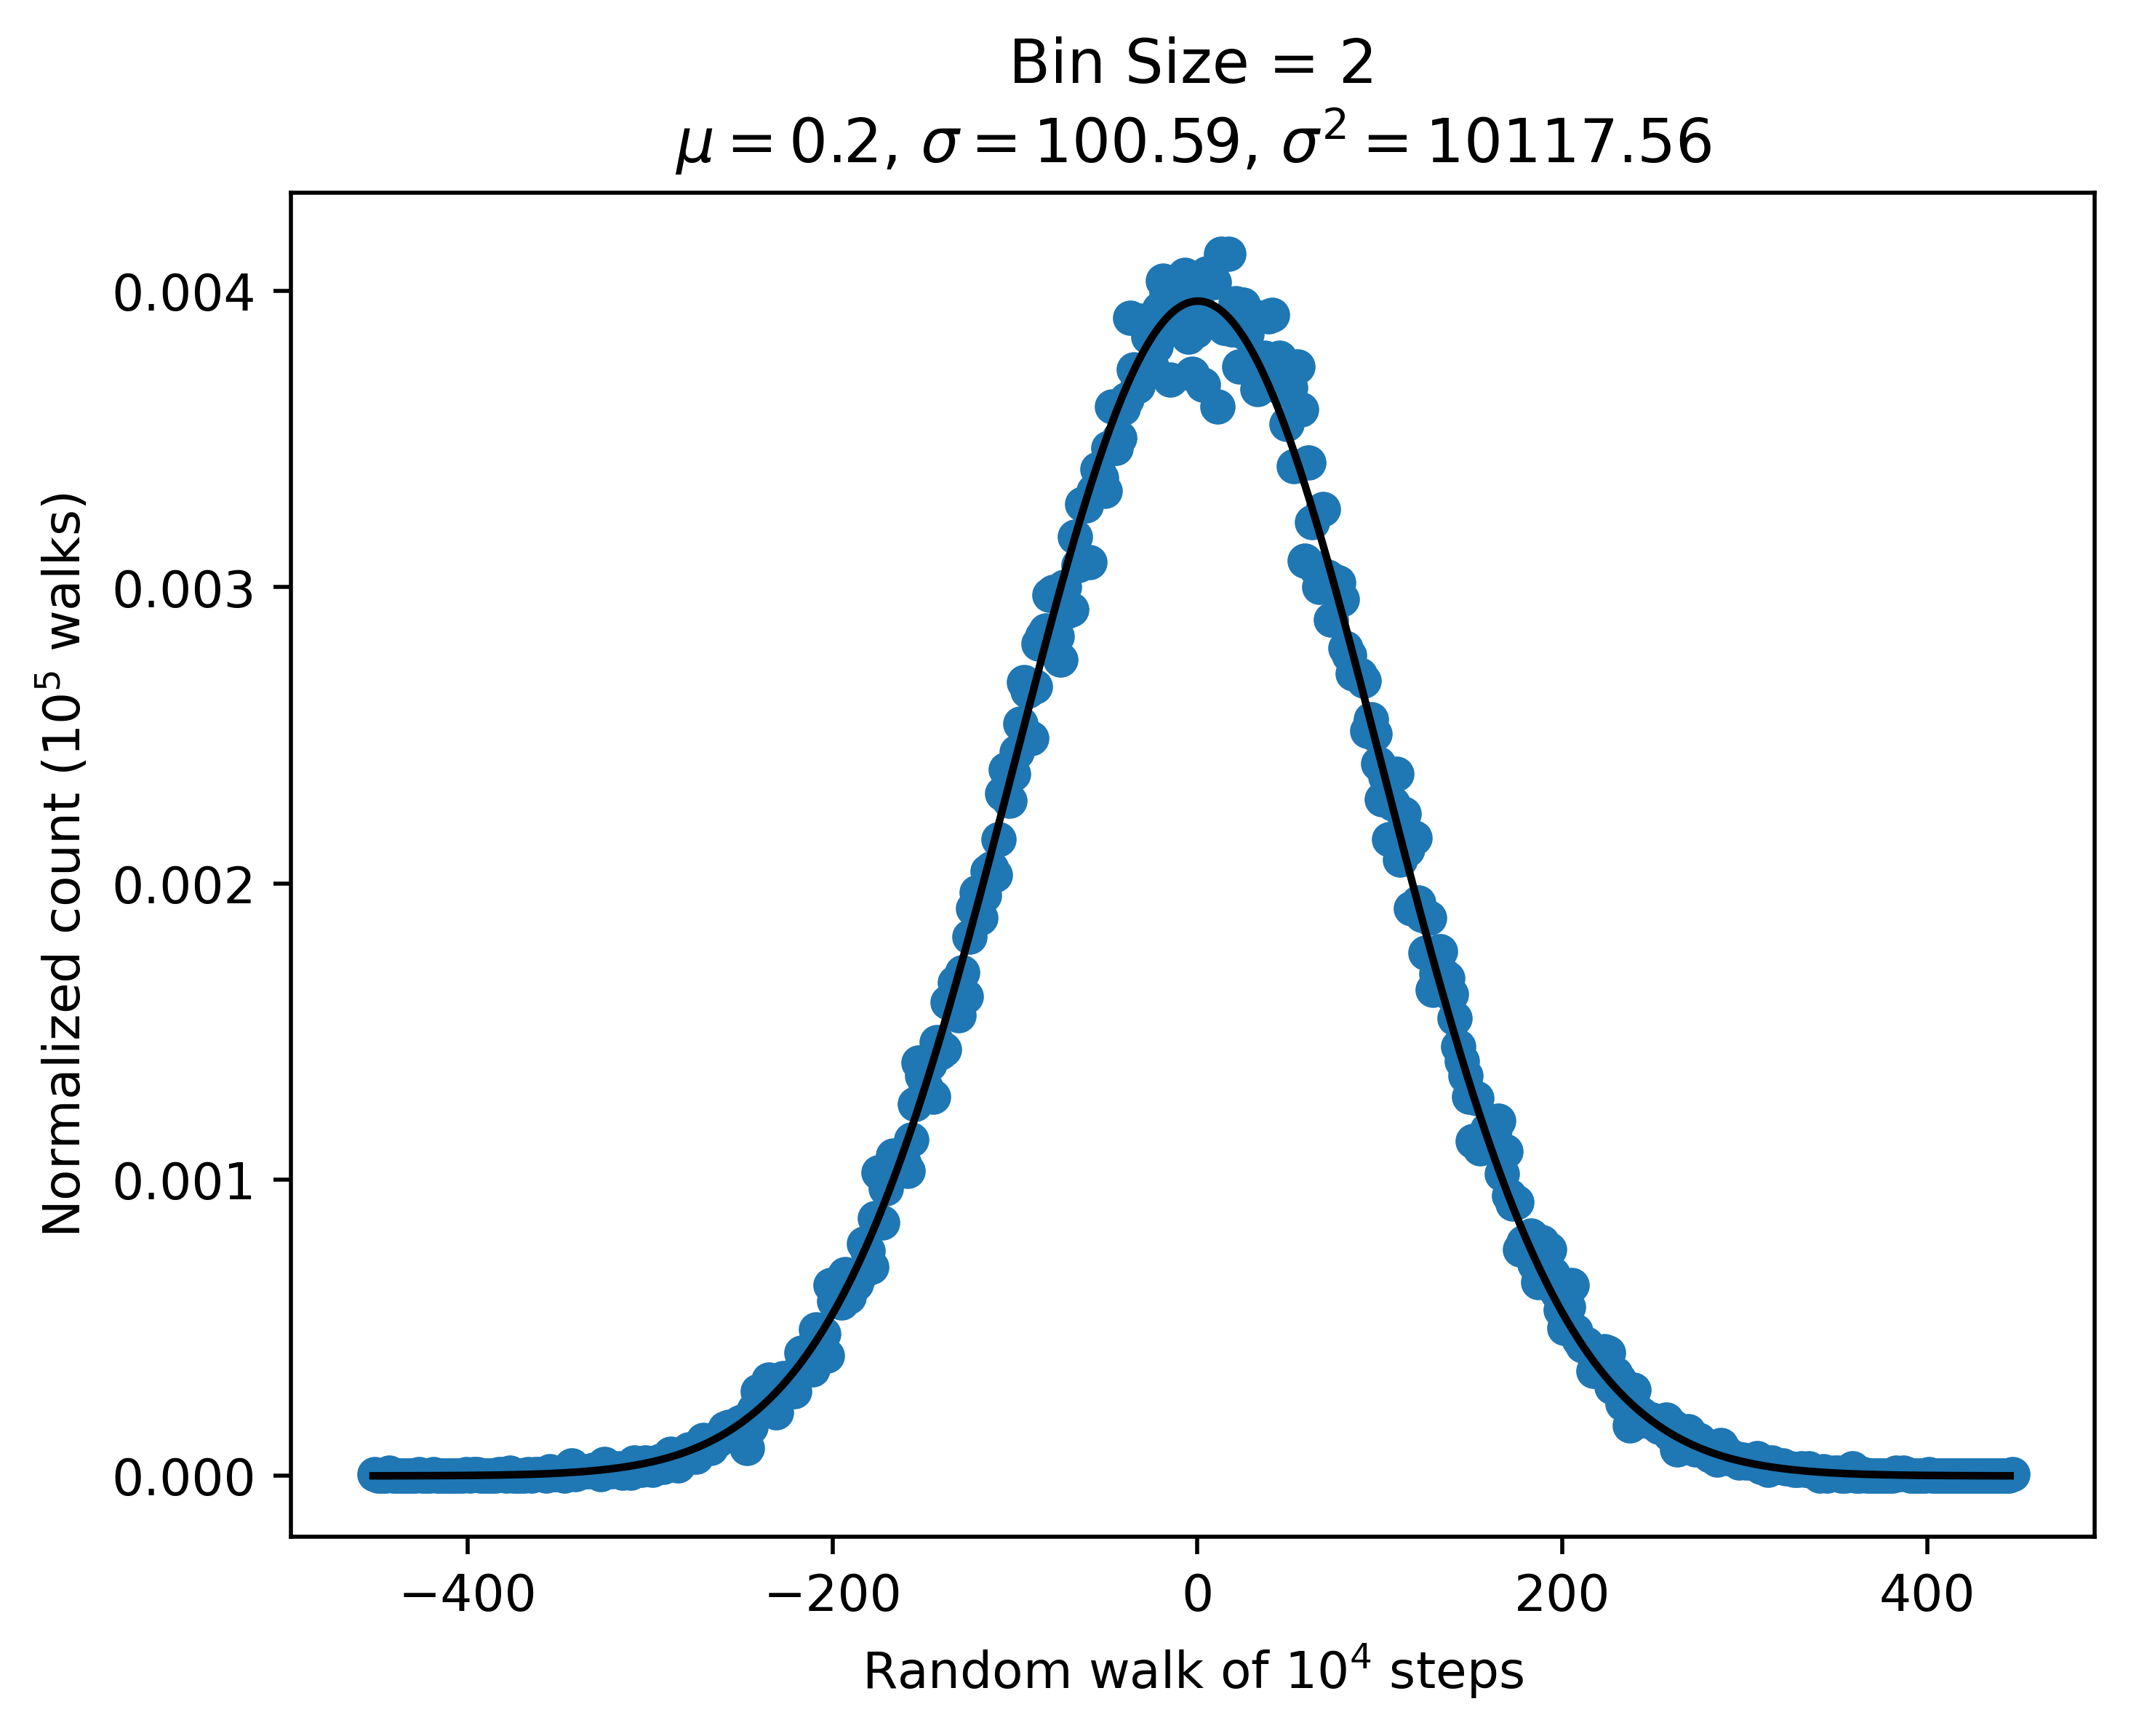
\includegraphics[scale=0.8]{1k.png}
\end{center}

\section*{1. l)}

\begin{center}
    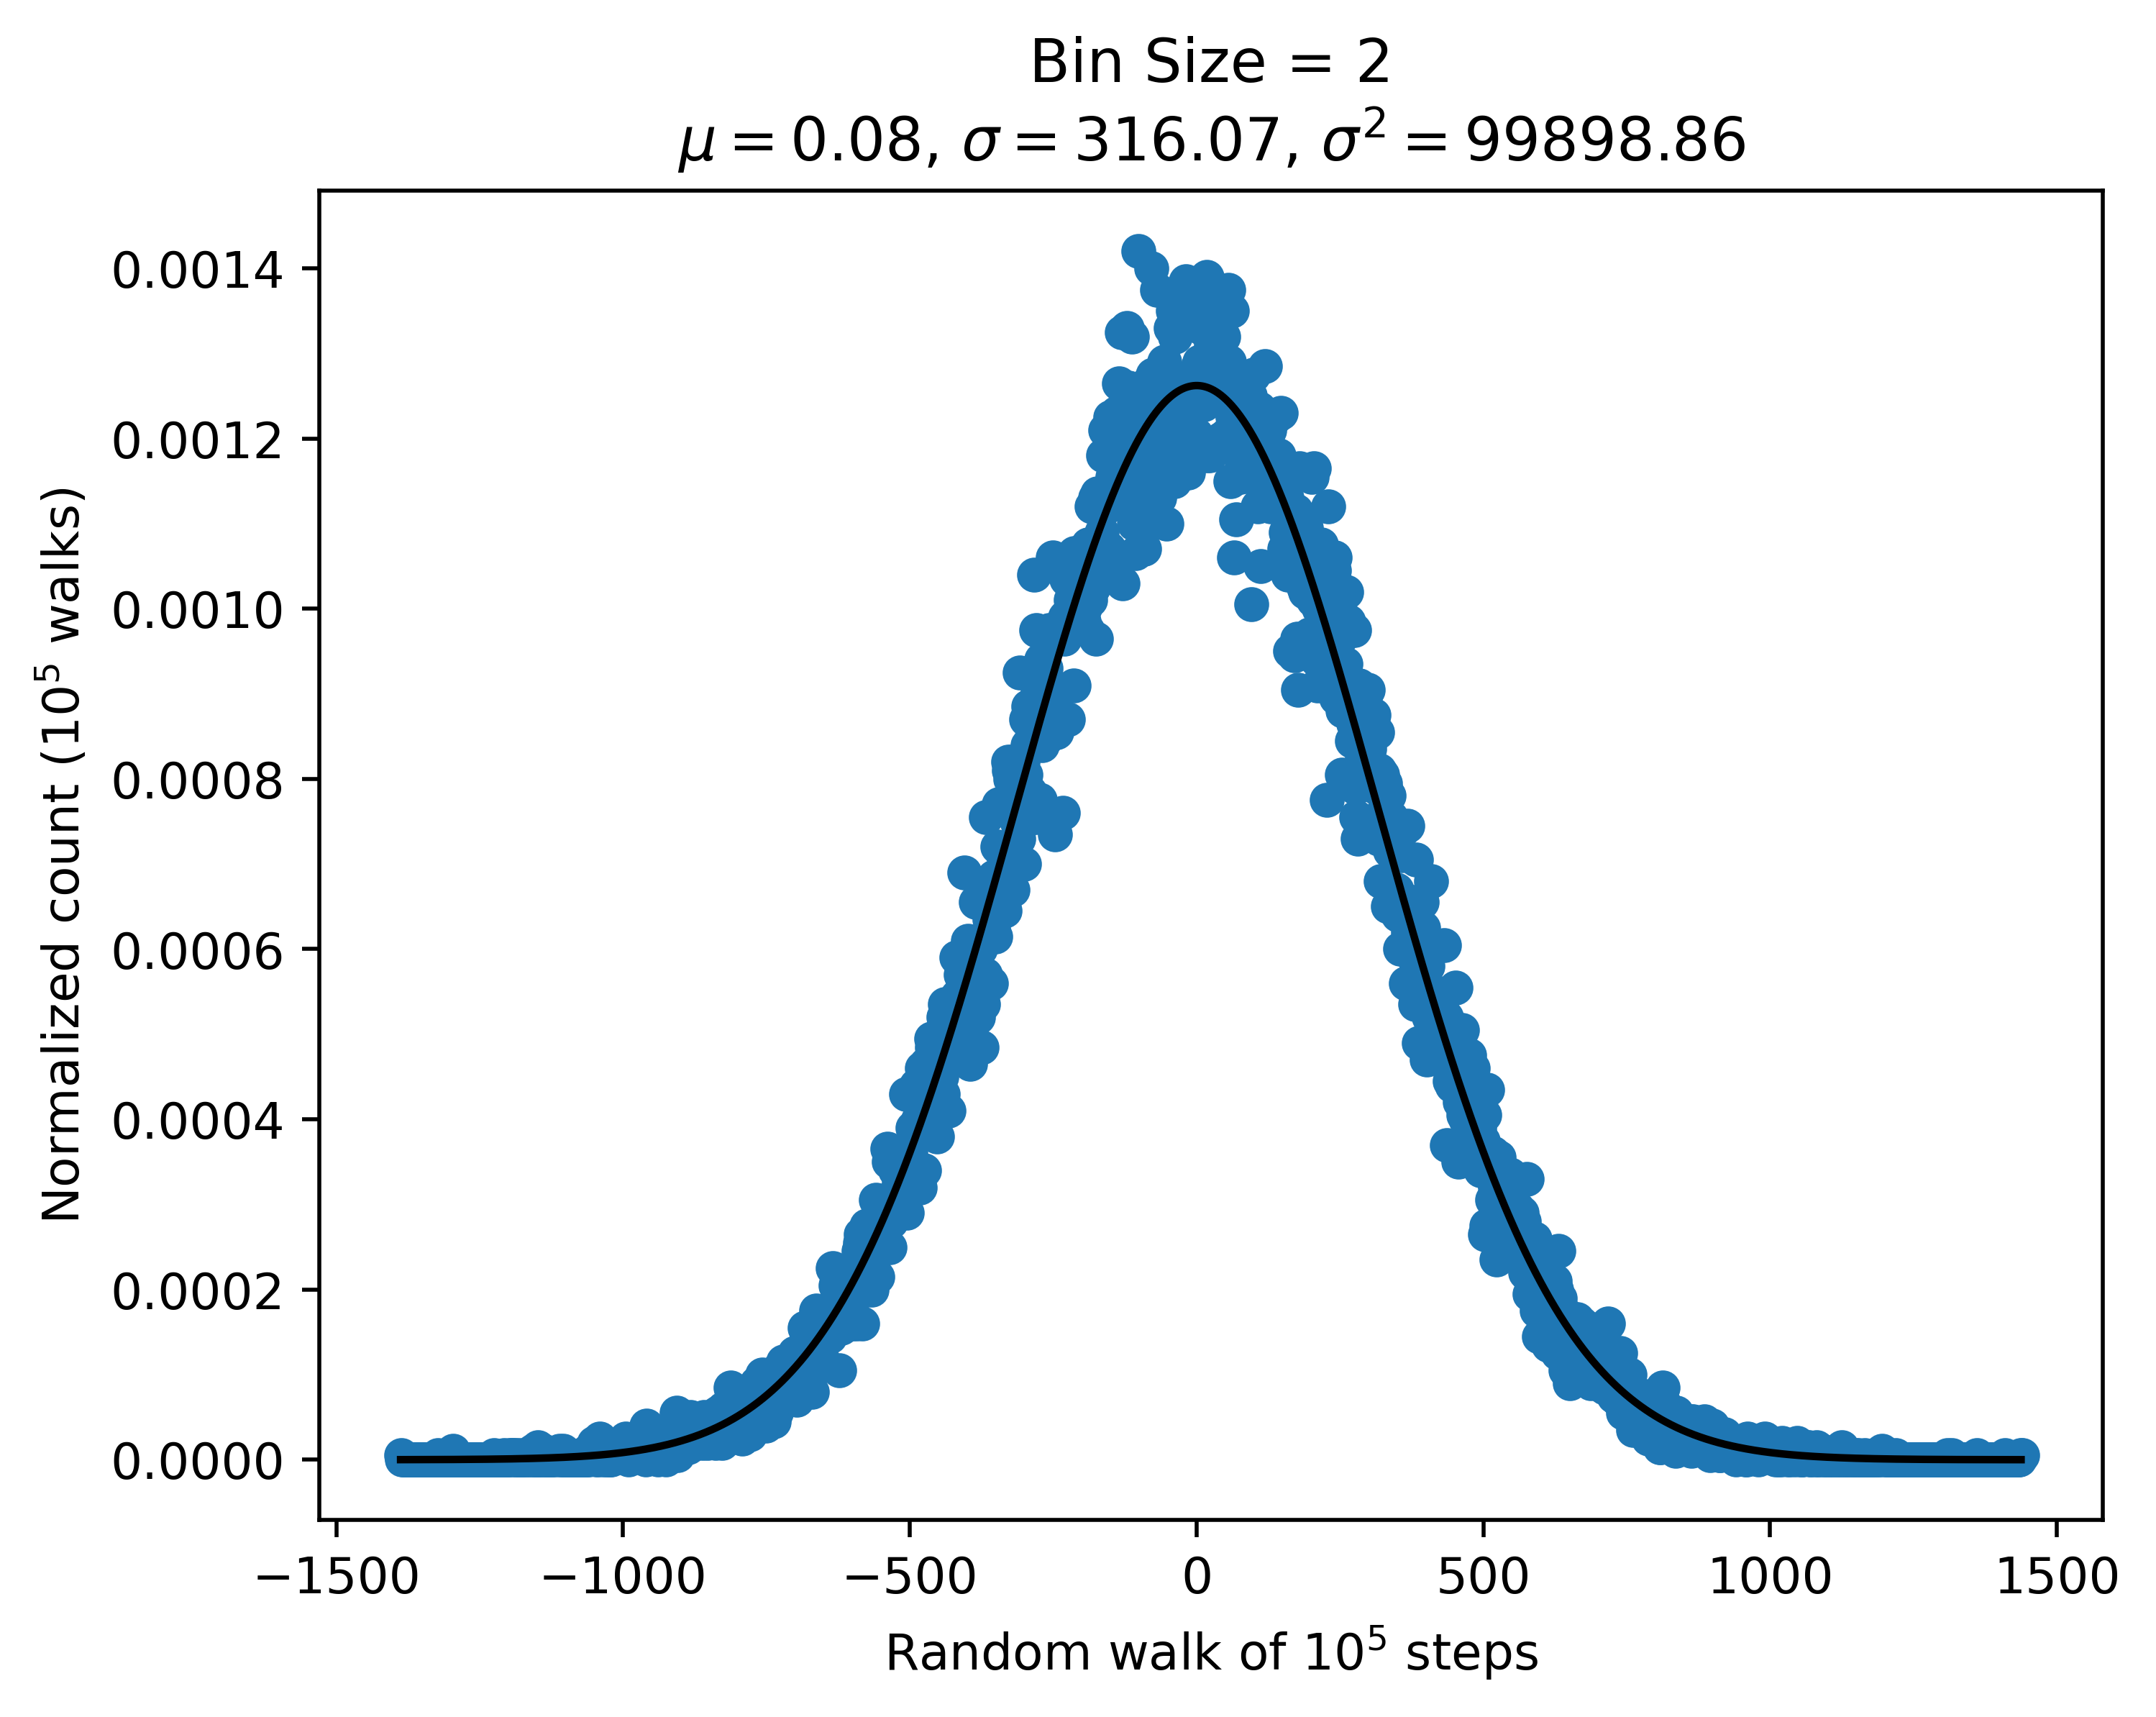
\includegraphics[scale=0.8]{1l.png}
\end{center}

\end{document}
